% Created 2020-03-08 Sun 11:35
% Intended LaTeX compiler: pdflatex
\documentclass[presentation]{beamer}
\usepackage[utf8]{inputenc}
\usepackage[T1]{fontenc}
\usepackage{graphicx}
\usepackage{grffile}
\usepackage{longtable}
\usepackage{wrapfig}
\usepackage{rotating}
\usepackage[normalem]{ulem}
\usepackage{amsmath}
\usepackage{textcomp}
\usepackage{amssymb}
\usepackage{capt-of}
\usepackage{hyperref}
\usepackage{awesomebox}
\usepackage{booktabs}
\usepackage{placeins}
\usepackage{siunitx}
\usepackage{minted}
\usetheme[progressbar=frametitle]{metropolis}
\usepackage{tikz}
\usetikzlibrary{backgrounds,matrix,fit,calc}
\usepackage{pgfplots}
\pgfplotsset{compat=1.16}
\usepackage{nicematrix}
\usepackage{spot}
\usepackage[beamer,customcolors]{hf-tikz}
\newcommand{\gv}[1]{\ensuremath{\mbox{\boldmath$ #1 $}}}
\newcommand{\bv}[1]{\ensuremath{\mathbf{#1}}}
\newcommand{\norm}[1]{\left\lVert#1\right\rVert}
\newcommand{\order}[1]{\mathcal O \left( #1 \right)} % order of magnitude
\newcommand*{\Scale}[2][4]{\scalebox{#1}{$#2$}}%
\definecolor{scarlet}{rgb}{1.0, 0.13, 0.0}
\definecolor{shamrockgreen}{rgb}{0.0, 0.62, 0.38}
\definecolor{royalblue}{rgb}{0.25, 0.41, 0.88}
\definecolor{metropolisorange}{RGB}{235,129,27}
\definecolor{deeppink}{RGB}{205,16,118}
\definecolor{burple}{RGB}{104,50,227}
\setmonofont{Iosevka Semibold}
\usetheme{default}
\author{\emph{Tejaswin Parthasarathy}, Mattia Gazzola}
\date{\today}
\title{Covariance Matrix Adaptation in Python}
\subtitle{ME498: Comp. modeling \& optimization}
\hypersetup{
 pdfauthor={\emph{Tejaswin Parthasarathy}, Mattia Gazzola},
 pdftitle={Covariance Matrix Adaptation in Python},
 pdfkeywords={},
 pdfsubject={},
 pdfcreator={Emacs 27.0.50 (Org mode 9.2)},
 pdflang={English}}
\begin{document}

\maketitle
\pgfplotsset{
colormap={whitered}{color(0cm)=(white); rgb255(1cm)=(235,129,27)}
}
\section{\texttt{Matplotlib}}
\label{sec:org2519178}
\begin{frame}[label={sec:org5253000},fragile]{Additional packages}
 \begin{itemize}
\item \texttt{Seaborn}  \alert{DEMO}
\item \texttt{bokeh}
\item \texttt{plotly}
\item See \href{https://wiki.python.org/moin/NumericAndScientific/Plotting}{Python wiki} for more plotting tools
\end{itemize}
\end{frame}
\begin{frame}[label={sec:org08882a5}]{Quick review}
\begin{block}{GA demo : Results of our GA implementation}
\end{block}
\begin{block}{How to improve convergence?}
\begin{itemize}
\item Parameters?
\item Strategies? (More mutation, less recombination say\ldots{}?)
\item Tuning is painful
\end{itemize}
\end{block}
\begin{block}{\(\Rightarrow\) CMAes (and other algorithms)}
\end{block}
\end{frame}
\section{Implementation of CMAes}
\label{sec:orgfc5a6a4}
\begin{frame}[label={sec:org2a3e2eb}]{The algorithm}
Set \(\mathbf{m} = \mathbf{0}, \mathbf{C} = \mathbf{I}, \sigma =
 0.5, \mathbf{p}_c = \mathbf{0}, \mathbf{p}_{\sigma} = \mathbf{0}\)
\begin{block}{Sampling}
\[ \begin{aligned}
	  \tikzmarkin<1>[set fill color=shamrockgreen!20, set border color=black]{sampling}(0.2,-0.4)(-0.2,0.6)
	  \mathbf{z}_{i} & \sim \mathcal{N}(\mathbf{0}, \mathbf{C}) \\
	  \mathbf{x}_{i} &= m+\sigma \mathbf{z}_{i} \tikzmarkend{sampling}
	  \end{aligned} \]
\end{block}

\begin{block}{Selection and Recombination}
\(\mu\) indicates best individuals
  \[ \begin{aligned}
	  \tikzmarkin<1>[set fill color=royalblue!40, set border color=black]{selec}(0.2,-0.4)(-0.2,0.8)
	  \langle\mathbf{z}\rangle_{w} &= \sum_{i=1}^{\mu} w_{i} \mathbf{z}_{i : \lambda} \\
	  \mathbf{m} &\longleftarrow \mathbf{m}+\sigma\langle\mathbf{z}\rangle_{w} \tikzmarkend{selec}
	  \end{aligned} \]
\end{block}
\end{frame}

\begin{frame}[label={sec:orge77186b}]{The algorithm contd.}
\begin{block}{Step size update}
\[ \begin{aligned}
	 \tikzmarkin<1>[set fill color=scarlet!30, set border color=black]{step}(5.2,-0.4)(-0.2,0.8)
	 \mathbf{p}_{\sigma} &\longleftarrow\left(1-c_{\sigma}\right)
	 \mathbf{p}_{\sigma}+\sqrt{1-\left(1-c_{\sigma}\right)^{2}}
	 \sqrt{\frac{1}{\sum_{i=1}^{\mu} w_{i}^{2}}}
	 \mathbf{C}^{-\frac{1}{2}}\langle\mathbf{z}\rangle_{w} \\
	 \sigma &\longleftarrow \sigma
	 e^{\left(\frac{1}{d_{\sigma}}\left(\frac{\left\|p_{\sigma}\right\|}{E\|\mathcal{N}(\mathbf{0},
	 \mathbf{I})\|}-1\right)\right)} \tikzmarkend{step}
	 \end{aligned} \]
\end{block}
\end{frame}

\begin{frame}[label={sec:orgf2cf930}]{The algorithm contd..}
\begin{block}{Covariance Matrix Update}
\[ \begin{aligned}
	   \tikzmarkin<1>[set fill color=metropolisorange!40, set border color=black]{cov}(0.4,-0.8)(-0.4,0.8)
	   \mathbf{p}_{c} &\longleftarrow \left(1-c_{c}\right)
	   \mathbf{p}_{c}+\sqrt{1-\left(1-c_{c}\right)^{2}} \sqrt{\frac{1}{\sum_{i=1}^{\mu}
	   w_{i}^{2}}}\langle\mathbf{z}\rangle_{w} \\
	   \mathbf{Z} &= \sum_{i=1}^{\mu} w_{i} \mathbf{z}_{i : \lambda} \mathbf{z}_{i :
	   \lambda}^{T} \\
	   \mu_{c o v}&=\sqrt{\frac{1}{\sum_{i=1}^{\mu} w_{i}^{2}}} \\
	   \mathbf{C} &\longleftarrow\left(1-c_{c o v}\right) \mathbf{C}+c_{c o v}
	   \frac{1}{\mu_{c o v}} \mathbf{p}_{c} \mathbf{p}_{c}^{T}+c_{c o
	   v}\left(1-\frac{1}{\mu_{c o v}}\right) \mathbf{Z} \tikzmarkend{cov}
	   \end{aligned} \]
\end{block}
\end{frame}
\begin{frame}[label={sec:org19751ac}]{Starting CMAes}
\begin{block}{Problem independent}
\begin{itemize}
\item Set evolution paths \(\gv{p}_\sigma = \gv{0}, \gv{p}_c = \gv{0}\)
\item Set number of generations \(g = 0\)
\item Set covariance matrix \(\bv{C} = \bv{I}\) (Why?)
\end{itemize}
\end{block}
\begin{block}{Problem dependent}
\begin{itemize}
\item Distribution mean \(\gv{m} \in \mathbb{R}^n\)
\item Step size \(\sigma \in \mathbb{R}_{>0}\) (Important to set \(>0\) )
\end{itemize}
\end{block}
\end{frame}
\begin{frame}[label={sec:org9fa580f}]{Starting CMAes: more on problem dependent parameters}
\begin{itemize}
\item Optimum presumably be within the initial cube \(\gv{m} \pm 3 \sigma
     \left(1 ,1 , \cdots, 1 \right)^T\)
\item \(\therefore\) if optima \(\in [a, b]^{n}\) choose \(\gv{m} \in [a,b]^{n}\) (as a uniformly random vector) and \(\sigma = 0.3*(b-a)\)
\item Different search intervals \(\Delta s_i\) for different variables can be
done using \(\bv{C}\) as shown below (deferred discussion):
\end{itemize}

\begin{equation}
\label{lyap_asym}
\begin{aligned}
\begin{bmatrix}
\Delta s^2_1 & 0 & \cdots & 0 \\
0 & \Delta s^2_2 & \cdots & 0 \\
\vdots & \ddots & \ddots & \vdots \\
0 & 0 &  \cdots & \Delta s^n_2  \\
\end{bmatrix}
\end{aligned}
\end{equation}

\begin{itemize}
\item \(\Delta s_i\) all must be of similar magnitude (for conditioning). Else,
rescale your problem.
\end{itemize}
\end{frame}
\begin{frame}[label={sec:org028cfa7},fragile]{First step : Sampling}
 \begin{block}{New population of points, for \(k = 1 \cdots \lambda\)}
\begin{itemize}
\item \(\gv{y}_k \sim \mathcal{N}\left( \gv{0}, \bv{I} \right)\)
\item \(\gv{z}_k \sim \mathcal{N}\left( \gv{0}, \bv{C} \right) =
     \bv{B}\bv{D}\gv{y}_k\)
\begin{itemize}
\item Given \(\bv{C} = \bv{B}\bv{D}^2\bv{B}^T\)
\item Consult \footnote{\url{https://math.stackexchange.com/q/2115701}}  for a proof of why \(\bv{A} \mathcal{N}\left(\gv{0}, \bv{I}
       \right) = \mathcal{N} \left(\gv{0}, \bv{A}\bv{A}^T \right)\)
\end{itemize}
\item \(\gv{x}_k = \gv{m} + \sigma \gv{z}_k \sim \mathcal{N}\left( \gv{m},
     \sigma^2 \bv{C} \right)\)
\end{itemize}
\end{block}
\begin{block}{Computing?}
\begin{itemize}
\item Steps 1 and 3 above using \texttt{*/np.multiply} for
elementwise multiplication and \texttt{+} for elementwise addition
\end{itemize}
\end{block}
\alert{We need a way to sample correlated (across dimensions) populations from} \texttt{numpy}
\end{frame}
\begin{frame}[label={sec:orgbccdcee},fragile]{Sampling : Python}
 \begin{block}{How to sample a multivariate normal distribution?}
\begin{itemize}
\item \texttt{np.random.multivariate\_normal} \alert{DEMO}
\end{itemize}
\end{block}
\begin{block}{Caveats?}
\begin{itemize}
\item What is \(\bv{C}\) / \texttt{cov} (in a 2D case) and its meaning?
\item \texttt{cov} needs to be SP(semi)D. Is it? What about the update step?
\item What happens in \texttt{numpy} if it is not?
\end{itemize}
\end{block}
\note{:B\_note:
\begin{itemize}
\item \(\mu_x = \frac{1}{N} \sum_{i=1}^{N}x_i\)
\item \(\sigma_x^2 = \frac{1}{N} \sum_{i=1}^{N}(x_i - \mu_x)^2\) and \(\sigma_{xy} = \frac{1}{N} \sum_{i=1}^{N}(x_i - \mu_x)(y_i - \mu_y)\)
\item Show symmetric nature of \texttt{cov} after update
\item Show positive definiteness (use PD of C, as well as the fact that it is
made up of rank-one decompositions
\item \texttt{numpy} checks for PD and throws an error
\item Now explain why you set \(A=CC^T\)
\end{itemize}}
\end{frame}
\begin{frame}[label={sec:orgf48683e}]{Normal Distribution\footnote{\href{https://upload.wikimedia.org/wikipedia/commons/2/25/The\_Normal\_Distribution.svg}{ Wikimedia Commons}}}
\begin{figure}[htbp]
\centering
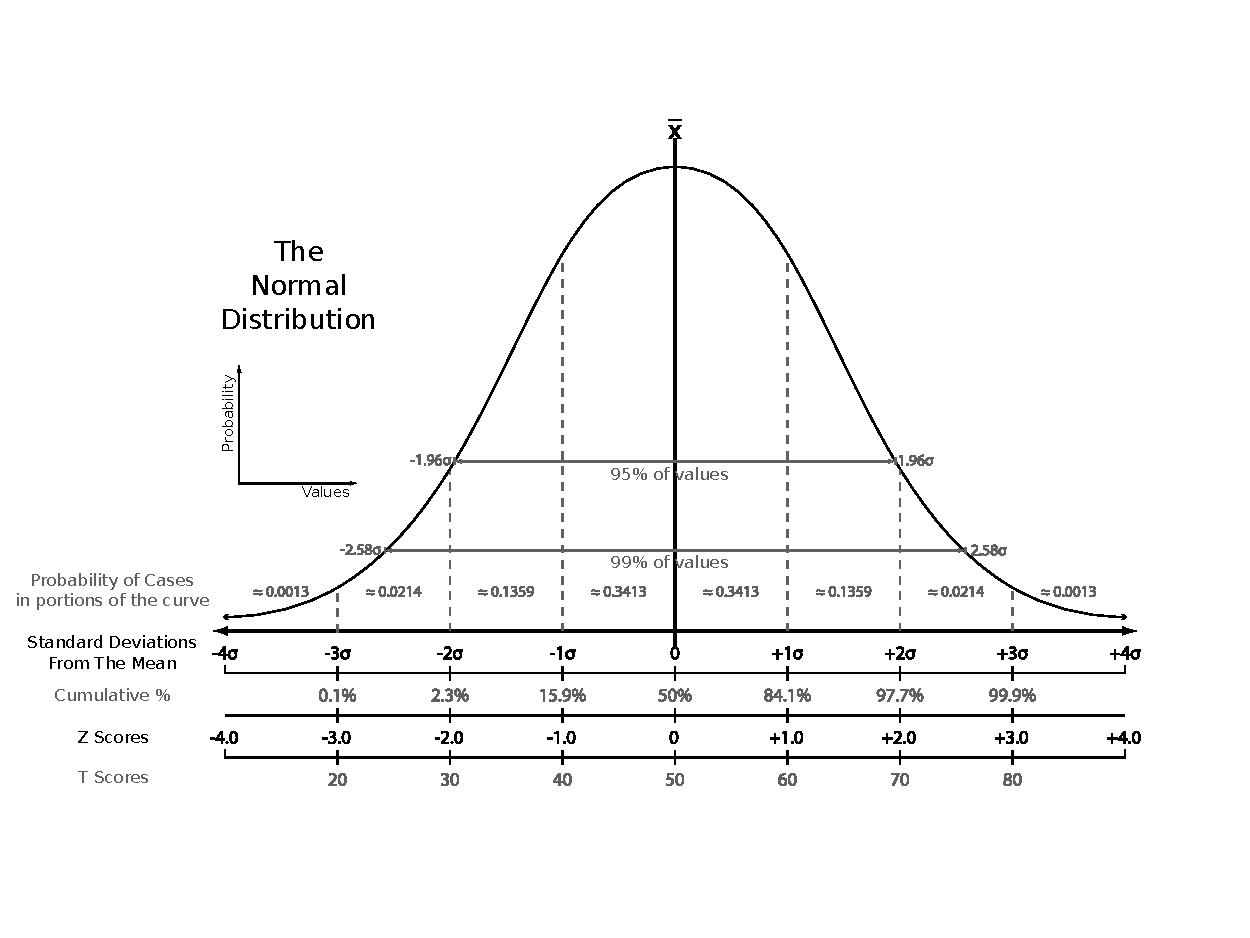
\includegraphics[width=.9\linewidth]{images/The_Normal_Distribution.pdf}
\caption{The Normal Distribution}
\end{figure}
\end{frame}
\begin{frame}[label={sec:org5f09065}]{Covariance Matrix \footnote{\href{https://www.slideshare.net/OsamaSalaheldin2/cmaes-presentation}{CMAes overview, Slideshare}}}
\begin{columns}
\begin{column}{0.5\columnwidth}
\begin{block}{\(\mathcal{N}(\gv{0}, \bv{I})\)}
\begin{center}
	\begin{tikzpicture}[
		declare function={mu1=0;},
		declare function={mu2=0;},
		declare function={sigma1=1;},
		declare function={sigma2=1;},
		declare function={normal(\m,\s)=1/(2*\s*sqrt(pi))*exp(-(x-\m)^2/(2*\s^2));},
		declare function={bivar(\ma,\sa,\mb,\sb)=
			1/(2*pi*\sa*\sb) * exp(-((x-\ma)^2/\sa^2 + (y-\mb)^2/\sb^2))/2;}, scale=0.6]
		\begin{axis}[
			colormap name=whitered,
			view={45}{65},
			enlargelimits=false,
			grid=major,
			domain=-2.5:2.5,
			y domain=-2.5:2.5,
			samples=26,
			xlabel=$x_1$,
			ylabel=$x_2$,
			zlabel={$\mathcal{N}$},
			colorbar,
			% colorbar style={
			% 	at={(1,0)},
			% 	anchor=south west,
			% 	height=0.25*\pgfkeysvalueof{/pgfplots/parent axis height},
			% 	title={$P(x_1,x_2)$}
			% }
		]
		\addplot3 [surf] {bivar(mu1,sigma1,mu2,sigma2)};
		\addplot3 [domain=-2.5:2.5,samples=31, samples y=0, thick, smooth] (x,2.5,{normal(mu1,sigma1)});
		\addplot3 [domain=-2.5:2.5,samples=31, samples y=0, thick, smooth] (-2.5,x,{normal(mu2,sigma2)});

		\draw [black!50] (axis cs:-2.5,0,0) -- (axis cs:2.5,0,0);
		\draw [black!50] (axis cs:0,-2.5,0) -- (axis cs:0,2.5,0);

		% \node at (axis cs:-1,1,0.18) [pin=165:$P(x_1)$] {};
		% \node at (axis cs:1.5,4,0.32) [pin=-15:$P(x_2)$] {};
		\end{axis}
	\end{tikzpicture}
\end{center}
\end{block}
\end{column}

\begin{column}{0.5\columnwidth}
\begin{block}{\(\mathcal{N}(\gv{\mu}, \bv{I})\)}
\begin{center}
	\begin{tikzpicture}[
		declare function={mu1=1;},
		declare function={mu2=-0.5;},
		declare function={sigma1=1;},
		declare function={sigma2=1;},
		declare function={normal(\m,\s)=1/(2*\s*sqrt(pi))*exp(-(x-\m)^2/(2*\s^2));},
		declare function={bivar(\ma,\sa,\mb,\sb)=
			1/(2*pi*\sa*\sb) * exp(-((x-\ma)^2/\sa^2 + (y-\mb)^2/\sb^2))/2;}, scale=0.6]
		\begin{axis}[
			colormap name=whitered,
			view={45}{65},
			enlargelimits=false,
			grid=major,
			domain=-2.5:2.5,
			y domain=-2.5:2.5,
			samples=26,
			xlabel=$x_1$,
			ylabel=$x_2$,
			zlabel={$\mathcal{N}$},
			colorbar,
		]
		\addplot3 [surf] {bivar(mu1,sigma1,mu2,sigma2)};
		\addplot3 [domain=-2.5:2.5,samples=31, samples y=0, thick, smooth] (x,2.5,{normal(mu1,sigma1)});
		\addplot3 [domain=-2.5:2.5,samples=31, samples y=0, thick, smooth] (-2.5,x,{normal(mu2,sigma2)});

		\draw [black!50] (axis cs:-2.5,0,0) -- (axis cs:2.5,0,0);
		\draw [black!50] (axis cs:0,-2.5,0) -- (axis cs:0,2.5,0);

		\end{axis}
	\end{tikzpicture}
\end{center}
\end{block}
\end{column}
\end{columns}
\note{:B\_note:
\begin{itemize}
\item Independence and identical distributions
\item Intution from Brad Osgood's notes on Fourier Transforms 3.7
\item End with CMA discovers the dependence and distribution of each random variable
\end{itemize}}
\end{frame}
\begin{frame}[label={sec:org7d3c819}]{Covariance Matrix}
\begin{columns}
\begin{column}{0.5\columnwidth}
\begin{block}{\(\mathcal{N}(\gv{0}, \bv{I})\)}
\begin{center}
	\begin{tikzpicture}[
		declare function={mu1=0;},
		declare function={mu2=0;},
		declare function={sigma1=1;},
		declare function={sigma2=1;},
		declare function={normal(\m,\s)=1/(2*\s*sqrt(pi))*exp(-(x-\m)^2/(2*\s^2));},
		declare function={bivar(\ma,\sa,\mb,\sb)=
			1/(2*pi*\sa*\sb) * exp(-((x-\ma)^2/\sa^2 + (y-\mb)^2/\sb^2))/2;}, scale=0.6]
		\begin{axis}[
			colormap name=whitered,
			view={45}{65},
			enlargelimits=false,
			grid=major,
			domain=-2.5:2.5,
			y domain=-2.5:2.5,
			samples=26,
			xlabel=$x_1$,
			ylabel=$x_2$,
			zlabel={$\mathcal{N}$},
			colorbar,
		]
		\addplot3 [surf] {bivar(mu1,sigma1,mu2,sigma2)};
		\addplot3 [domain=-2.5:2.5,samples=31, samples y=0, thick, smooth] (x,2.5,{normal(mu1,sigma1)});
		\addplot3 [domain=-2.5:2.5,samples=31, samples y=0, thick, smooth] (-2.5,x,{normal(mu2,sigma2)});

		\draw [black!50] (axis cs:-2.5,0,0) -- (axis cs:2.5,0,0);
		\draw [black!50] (axis cs:0,-2.5,0) -- (axis cs:0,2.5,0);
		\end{axis}
	\end{tikzpicture}
\end{center}
\end{block}
\end{column}

\begin{column}{0.5\columnwidth}
\begin{block}{\(\mathcal{N}(\gv{0}, \bv{C})\)}
\begin{center}
	\begin{tikzpicture}[
		declare function={mu1=0;},
		declare function={mu2=0;},
		declare function={sigma1=0.5;},
		declare function={sigma2=2;},
		declare function={normal(\m,\s)=1/(2*\s*sqrt(pi))*exp(-(x-\m)^2/(2*\s^2));},
		declare function={bivar(\ma,\sa,\mb,\sb)=
			1/(2*pi*\sa*\sb) * exp(-(((x*cos(60) + y*sin(60))-\ma)^2/\sa^2 + ((-x*sin(60) + y*cos(60))-\mb)^2/\sb^2))/2;}, scale=0.6]
		\begin{axis}[
			colormap name=whitered,
			view={45}{65},
			enlargelimits=false,
			grid=major,
			domain=-2.5:2.5,
			y domain=-2.5:2.5,
			samples=26,
			xlabel=$x_1$,
			ylabel=$x_2$,
			zlabel={$\mathcal{N}$},
			colorbar,
		]
		\addplot3 [surf] {bivar(mu1,sigma1,mu2,sigma2)};
		% \addplot3 [domain=-2.5:2.5,samples=31, samples y=0, thick, smooth] (x,2.5,{normal(mu1,sigma1)});
		% \addplot3 [domain=-2.5:2.5,samples=31, samples y=0, thick, smooth] (-2.5,x,{normal(mu2,sigma2)});

		\draw [black!50] (axis cs:-2.5,0,0) -- (axis cs:2.5,0,0);
		\draw [black!50] (axis cs:0,-2.5,0) -- (axis cs:0,2.5,0);

		\end{axis}
	\end{tikzpicture}
\end{center}
\end{block}
\end{column}
\end{columns}
\end{frame}
\begin{frame}[label={sec:orga9ef288}]{Covariance Matrix : Example 1}
\[ \bv{C} = \begin{bmatrix} 1 & 0 \\ 0 & 1\end{bmatrix}\]
\begin{columns}
\begin{column}{0.5\columnwidth}
\begin{center}
	\begin{tikzpicture}[
		declare function={mu1=0;},
		declare function={mu2=0;},
		declare function={sigma1=1;},
		declare function={sigma2=1;},
		declare function={normal(\m,\s)=1/(2*\s*sqrt(pi))*exp(-(x-\m)^2/(2*\s^2));},
		declare function={bivar(\ma,\sa,\mb,\sb)=
			1/(2*pi*\sa*\sb) * exp(-((x-\ma)^2/\sa^2 + (y-\mb)^2/\sb^2))/2;}, scale=0.6, baseline]
		\begin{axis}[
			colormap name=whitered,
			view={45}{65},
			enlargelimits=false,
			grid=major,
			domain=-2.5:2.5,
			y domain=-2.5:2.5,
			samples=26,
			xlabel=$x_1$,
			ylabel=$x_2$,
			zlabel={$\mathcal{N}$},
			colorbar,
		]
		\addplot3 [surf] {bivar(mu1,sigma1,mu2,sigma2)};
		\addplot3 [domain=-2.5:2.5,samples=31, samples y=0, thick, smooth] (x,2.5,{normal(mu1,sigma1)});
		\addplot3 [domain=-2.5:2.5,samples=31, samples y=0, thick, smooth] (-2.5,x,{normal(mu2,sigma2)});

		\draw [black!50] (axis cs:-2.5,0,0) -- (axis cs:2.5,0,0);
		\draw [black!50] (axis cs:0,-2.5,0) -- (axis cs:0,2.5,0);
		\end{axis}
	\end{tikzpicture}
\end{center}
\end{column}
\begin{column}{0.5\columnwidth}
\begin{center}
	\begin{tikzpicture}[baseline,scale=0.6]
		\begin{axis}[
			enlargelimits=false,
			grid=major,
			ymin=-2.5, ymax=2.5,
			xmin=-2.5, xmax=2.5,
			xlabel=$x_1$,
			ylabel=$x_2$,
		]
		\addplot [only marks, mark=*,
		mark size=2.5pt, metropolisorange, mark options={fill=metropolisorange}] table {data/normal.txt};

		\draw [black!50] (axis cs:-2.5,0,0) -- (axis cs:2.5,0,0);
		\draw [black!50] (axis cs:0,-2.5,0) -- (axis cs:0,2.5,0);

		\end{axis}
	\end{tikzpicture}
\end{center}
\end{column}
\end{columns}
\end{frame}
\begin{frame}[label={sec:org96fb544}]{Covariance Matrix : Example 2}
\[ \bv{C} = \begin{bmatrix} 1 & 0 \\ 0 & \spot{0.2}\end{bmatrix}\]
\begin{columns}
\begin{column}{0.5\columnwidth}
\begin{center}
	\begin{tikzpicture}[
		declare function={mu1=0;},
		declare function={mu2=0;},
		declare function={sigma1=1;},
		declare function={sigma2=0.2;},
		declare function={normal(\m,\s)=1/(2*\s*sqrt(pi))*exp(-(x-\m)^2/(2*\s^2));},
		declare function={bivar(\ma,\sa,\mb,\sb)=
			1/(2*pi*\sa*\sb) * exp(-((x-\ma)^2/\sa^2 + (y-\mb)^2/\sb^2))/2;}, scale=0.6, baseline]
		\begin{axis}[
			colormap name=whitered,
			view={45}{65},
			enlargelimits=false,
			grid=major,
			domain=-2.5:2.5,
			y domain=-2.5:2.5,
			samples=26,
			xlabel=$x_1$,
			ylabel=$x_2$,
			zlabel={$\mathcal{N}$},
			colorbar,
		]
		\addplot3 [surf] {bivar(mu1,sigma1,mu2,sigma2)};
		\addplot3 [domain=-2.5:2.5,samples=31, samples y=0, thick, smooth] (x,2.5,{normal(mu1,sigma1)});
		\addplot3 [domain=-2.5:2.5,samples=31, samples y=0, thick, smooth] (-2.5,x,{normal(mu2,sigma2)});

		\draw [black!50] (axis cs:-2.5,0,0) -- (axis cs:2.5,0,0);
		\draw [black!50] (axis cs:0,-2.5,0) -- (axis cs:0,2.5,0);

		\end{axis}
	\end{tikzpicture}
\end{center}
\end{column}

\begin{column}{0.5\columnwidth}
\begin{center}
	\begin{tikzpicture}[baseline,scale=0.6]
		\begin{axis}[
			enlargelimits=false,
			grid=major,
			ymin=-2.5, ymax=2.5,
			xmin=-2.5, xmax=2.5,
			xlabel=$x_1$,
			ylabel=$x_2$,
		]
		\addplot [only marks, mark=*,
		mark size=2.5pt, metropolisorange, mark options={fill=metropolisorange}] table {data/skewedX.txt};

		\draw [black!50] (axis cs:-2.5,0,0) -- (axis cs:2.5,0,0);
		\draw [black!50] (axis cs:0,-2.5,0) -- (axis cs:0,2.5,0);

		\end{axis}
	\end{tikzpicture}
\end{center}
\end{column}
\end{columns}
\end{frame}
\begin{frame}[label={sec:orga0d4e7e}]{Covariance Matrix : Example 3}
\[ \bv{C} = \begin{bmatrix} \spot{0.2} & 0 \\ 0 & 1\end{bmatrix}\]
\begin{columns}
\begin{column}{0.5\columnwidth}
\begin{center}
	\begin{tikzpicture}[
		declare function={mu1=0;},
		declare function={mu2=0;},
		declare function={sigma1=0.2;},
		declare function={sigma2=1.0;},
		declare function={normal(\m,\s)=1/(2*\s*sqrt(pi))*exp(-(x-\m)^2/(2*\s^2));},
		declare function={bivar(\ma,\sa,\mb,\sb)=
			1/(2*pi*\sa*\sb) * exp(-((x-\ma)^2/\sa^2 + (y-\mb)^2/\sb^2))/2;}, scale=0.6, baseline]
		\begin{axis}[
			colormap name=whitered,
			view={45}{65},
			enlargelimits=false,
			grid=major,
			domain=-2.5:2.5,
			y domain=-2.5:2.5,
			samples=26,
			xlabel=$x_1$,
			ylabel=$x_2$,
			zlabel={$\mathcal{N}$},
			colorbar,
		]
		\addplot3 [surf] {bivar(mu1,sigma1,mu2,sigma2)};
		\addplot3 [domain=-2.5:2.5,samples=31, samples y=0, thick, smooth] (x,2.5,{normal(mu1,sigma1)});
		\addplot3 [domain=-2.5:2.5,samples=31, samples y=0, thick, smooth] (-2.5,x,{normal(mu2,sigma2)});

		\draw [black!50] (axis cs:-2.5,0,0) -- (axis cs:2.5,0,0);
		\draw [black!50] (axis cs:0,-2.5,0) -- (axis cs:0,2.5,0);

		\end{axis}
	\end{tikzpicture}
\end{center}
\end{column}

\begin{column}{0.5\columnwidth}
\begin{center}
	\begin{tikzpicture}[baseline,scale=0.6]
		\begin{axis}[
			enlargelimits=false,
			grid=major,
			ymin=-2.5, ymax=2.5,
			xmin=-2.5, xmax=2.5,
			xlabel=$x_1$,
			ylabel=$x_2$,
		]
		\addplot [only marks, mark=*,
		mark size=2.5pt, metropolisorange, mark options={fill=metropolisorange}] table {data/skewedY.txt};

		\draw [black!50] (axis cs:-2.5,0,0) -- (axis cs:2.5,0,0);
		\draw [black!50] (axis cs:0,-2.5,0) -- (axis cs:0,2.5,0);

		\end{axis}
	\end{tikzpicture}
\end{center}
\end{column}
\end{columns}
\end{frame}
\begin{frame}[label={sec:org42bc1ad}]{Covariance Matrix : Example 4}
\[ \bv{C} = \begin{bmatrix} 0.2 & \spot{0.36} \\ \spot{0.36} & 1\end{bmatrix}\]
\begin{columns}
\begin{column}{0.5\columnwidth}
\begin{center}
	\begin{tikzpicture}[
		declare function={mu1=0;},
		declare function={mu2=0;},
		declare function={sigma1=0.2;},
		declare function={sigma2=1.0;},
		declare function={normal(\m,\s)=1/(2*\s*sqrt(pi))*exp(-(x-\m)^2/(2*\s^2));},
		declare function={bivar(\ma,\sa,\mb,\sb)=
			1/(2*pi*\sa*\sb) * exp(-(((-0.35826*x - 0.93362*y)-\ma)^2/\sa^2 + ((-0.93362*x + 0.358266*y)-\mb)^2/\sb^2))/2;}, scale=0.6, baseline]
		\begin{axis}[
			colormap name=whitered,
			view={45}{65},
			enlargelimits=false,
			grid=major,
			domain=-2.5:2.5,
			y domain=-2.5:2.5,
			samples=26,
			xlabel=$x_1$,
			ylabel=$x_2$,
			zlabel={$\mathcal{N}$},
			colorbar,
		]
		\addplot3 [surf] {bivar(mu1,sigma1,mu2,sigma2)};
		%\addplot3 [domain=-2.5:2.5,samples=31, samples y=0, thick, smooth] (x,2.5,{normal(mu1,sigma1)});
		%\addplot3 [domain=-2.5:2.5,samples=31, samples y=0, thick, smooth] (-2.5,x,{normal(mu2,sigma2)});

		\draw [black!50] (axis cs:-2.5,0,0) -- (axis cs:2.5,0,0);
		\draw [black!50] (axis cs:0,-2.5,0) -- (axis cs:0,2.5,0);

		\end{axis}
	\end{tikzpicture}
\end{center}
\end{column}

\begin{column}{0.5\columnwidth}
\begin{center}
	\begin{tikzpicture}[baseline,scale=0.6]
		\begin{axis}[
			enlargelimits=false,
			grid=major,
			ymin=-2.5, ymax=2.5,
			xmin=-2.5, xmax=2.5,
			xlabel=$x_1$,
			ylabel=$x_2$,
		]
		\addplot [only marks, mark=*,
		mark size=2.5pt, metropolisorange, mark options={fill=metropolisorange}] table {data/skewedXY.txt};

		\draw [black!50] (axis cs:-2.5,0,0) -- (axis cs:2.5,0,0);
		\draw [black!50] (axis cs:0,-2.5,0) -- (axis cs:0,2.5,0);

		\end{axis}
	\end{tikzpicture}
\end{center}
\end{column}
\end{columns}
\end{frame}
\begin{frame}[label={sec:org4de67dc}]{Covariance Matrix : Definition}
Covariance Matrix decides the ``direction'' of the population\ldots{}

\[ \left(\,\begin{NiceArray}{>{\strut}CCCC}%
   [create-extra-nodes,left-margin,right-margin,
   code-after = {\tikz \path [name suffix = -large,
   fill = metropolisorange!40,
   blend mode = multiply]
   (1-2.north west)|- (2-3.north west)|- (3-4.north west)|-
   (3-4.south east)|- (1-2.north west) ;
   \tikz \path [name suffix = -large,
   fill = metropolisorange!40,
   blend mode = multiply]
   (2-1.north west)|- (4-1.south west)|- (4-3.south east)|-
   (4-3.north west)|- (3-2.north west)|- (2-1.north west) ;
   \tikz \path [name suffix = -large,
   fill = royalblue!60,
   blend mode = multiply]
   (1-1.north west)|- (2-2.north west)|- (3-3.north west)|-
   (4-4.north west)|- (4-4.south east)|- (4-4.north west)|-
   (3-3.north west)|- (2-2.north west)|- (1-1.north west);} ]
   C_{11} & C_{12} & C_{13} & C_{14} \\C_{21} & C_{22} & C_{23} & C_{24} \\C_{31} & C_{32} & C_{33} & C_{34} \\C_{41} & C_{42} & C_{43} & C_{44}\end{NiceArray}\,
   \right)\]

\tikz{\draw[fill=royalblue!60,line width=1pt]  rectangle(4ex, 2ex);}  \(\rightarrow\) Variance

\tikz{\draw[fill=metropolisorange!40,line width=1pt]  rectangle(4ex, 2ex);}  \(\rightarrow\) Covariance

Nonzero covariances \(\Rightarrow\) Population is not iid and is skewed wrt
coordinate axes.
\end{frame}

\begin{frame}[label={sec:org6cb13e6}]{Variance}
\begin{definition}[Variance]
\(\sigma^2\) Is a measure of how ``far'' a variable changes away from its mean.
\end{definition}

\[ \sigma^2  = \frac{1}{N} \sum_{i=1}^{N}(x_i - \mu)^2 \]
where \(\mu\) is the mean and \(N\) is the number of samples.
\end{frame}

\begin{frame}[label={sec:orge95c720}]{Variance}
\begin{example}[Low variance]
\begin{center}
	\begin{tikzpicture}[baseline,scale=0.9]
		\begin{axis}[
			% only scale the axis, not the axis including the ticks and labels
			scale only axis=true,
			% set `width' and `height' to the desired values
			width=0.7\textwidth,
			height=0.2\textwidth,
			enlargelimits=true,
			grid=major,
			xlabel=$i$,
			ylabel=$x_i$,
			ymin=-2.5,ymax=2.5,
			xticklabels={,,},
		]
		\addplot [only marks, mark=*,
		mark size=2.5pt, metropolisorange, mark options={fill=metropolisorange}] table {data/lowvar.txt};
		\draw[thick, black] (axis cs:\pgfkeysvalueof{/pgfplots/xmin},0) -- (axis cs:\pgfkeysvalueof{/pgfplots/xmax},0) node[left,pos=1] (endofplot){};
		\node [above] at (endofplot) {$\mu$};
		\end{axis}
	\end{tikzpicture}
\end{center}
\end{example}

\begin{example}[High variance]
\begin{center}
	\begin{tikzpicture}[baseline,scale=0.9]
		\begin{axis}[
			% only scale the axis, not the axis including the ticks and labels
			scale only axis=true,
			% set `width' and `height' to the desired values
			width=0.7\textwidth,
			height=0.2\textwidth,
			enlargelimits=true,
			grid=major,
			xlabel=$i$,
			ylabel=$x_i$,
			ymin=-2.5,ymax=2.5,
			xticklabels={,,},
		]
		\addplot [only marks, mark=*,
		mark size=2.5pt, metropolisorange, mark options={fill=metropolisorange}] table {data/highvar.txt};
		\draw[thick, black] (axis cs:\pgfkeysvalueof{/pgfplots/xmin},0) -- (axis cs:\pgfkeysvalueof{/pgfplots/xmax},0) node[left,pos=1] (endofplot){};
		\node [above] at (endofplot) {$\mu$};
		\end{axis}
	\end{tikzpicture}
\end{center}
\end{example}
\end{frame}
\begin{frame}[label={sec:orga34118a}]{Covariance}
\begin{definition}[Covariance]
covar\((x,y)\) Is a measure of how two variables change with one another.
\end{definition}

\[ \sigma_{xy} = \frac{1}{N} \sum_{i=1}^{N}(x_i - \mu_x)(y_i - \mu_y) \]
where \(\mu_x, \mu_y\) are the respective means and \(N\) is the number of samples.
\end{frame}

\begin{frame}[label={sec:org5251322}]{Covariance}
\begin{example}[Covariance (x,y,z)]
\begin{center}
	\begin{tikzpicture}[baseline]
		\begin{axis}[
			% only scale the axis, not the axis including the ticks and labels
			scale only axis=true,
			% set `width' and `height' to the desired values
			width=0.7\textwidth,
			height=0.12\textwidth,
			enlargelimits=true,
			grid=major,
			ylabel=$x_i$,
			ymin=-1.0,ymax=1.0,
			xticklabels={,,},
		]
		\addplot [only marks, mark=*,
		mark size=2.5pt, metropolisorange, mark options={fill=metropolisorange}] table {data/orig.txt};
		\draw[thick, black] (axis cs:\pgfkeysvalueof{/pgfplots/xmin},0) -- (axis cs:\pgfkeysvalueof{/pgfplots/xmax},0) node[left,pos=1] (endofplot){};
		\node [above] at (endofplot) {$\mu_x$};
		\end{axis}
	\end{tikzpicture}
\end{center}

\begin{center}
	\begin{tikzpicture}[baseline]
		\begin{axis}[
			% only scale the axis, not the axis including the ticks and labels
			scale only axis=true,
			% set `width' and `height' to the desired values
			width=0.7\textwidth,
			height=0.12\textwidth,
			enlargelimits=true,
			grid=major,
			ylabel=$y_i$,
			ymin=-1.0,ymax=1.0,
			xticklabels={,,},
		]
		\addplot [only marks, mark=*,
		mark size=2.5pt, metropolisorange, mark options={fill=metropolisorange}] table {data/poscovar.txt};
		\draw[thick, black] (axis cs:\pgfkeysvalueof{/pgfplots/xmin},0) -- (axis cs:\pgfkeysvalueof{/pgfplots/xmax},0) node[left,pos=1] (endofplot){};
		\node [above] at (endofplot) {$\mu_y$};
		\end{axis}
	\end{tikzpicture}
\end{center}

\begin{center}
	\begin{tikzpicture}[baseline]
		\begin{axis}[
			% only scale the axis, not the axis including the ticks and labels
			scale only axis=true,
			% set `width' and `height' to the desired values
			width=0.7\textwidth,
			height=0.12\textwidth,
			enlargelimits=true,
			grid=major,
			xlabel=$i$,
			ylabel=$z_i$,
			ymin=-1.0,ymax=1.0,
			xticklabels={,,},
		]
		\addplot [only marks, mark=*,
		mark size=2.5pt, metropolisorange, mark options={fill=metropolisorange}] table {data/negcovar.txt};
		\draw[thick, black] (axis cs:\pgfkeysvalueof{/pgfplots/xmin},0) -- (axis cs:\pgfkeysvalueof{/pgfplots/xmax},0) node[left,pos=1] (endofplot){};
		\node [above] at (endofplot) {$\mu_z$};
		\end{axis}
	\end{tikzpicture}
\end{center}
\end{example}
\end{frame}
\begin{frame}[label={sec:orgd43416a}]{Covariance Matrix : Definition}
Covariance Matrix decides the ``direction'' of the population\ldots{}

\[ \left(\,\begin{NiceArray}{>{\strut}CCCC}%
   [create-extra-nodes,left-margin,right-margin,
   code-after = {\tikz \path [name suffix = -large,
   fill = metropolisorange!40,
   blend mode = multiply]
   (1-2.north west)|- (2-3.north west)|- (3-4.north west)|-
   (3-4.south east)|- (1-2.north west) ;
   \tikz \path [name suffix = -large,
   fill = metropolisorange!40,
   blend mode = multiply]
   (2-1.north west)|- (4-1.south west)|- (4-3.south east)|-
   (4-3.north west)|- (3-2.north west)|- (2-1.north west) ;
   \tikz \path [name suffix = -large,
   fill = royalblue!60,
   blend mode = multiply]
   (1-1.north west)|- (2-2.north west)|- (3-3.north west)|-
   (4-4.north west)|- (4-4.south east)|- (4-4.north west)|-
   (3-3.north west)|- (2-2.north west)|- (1-1.north west);} ]
   C_{11} & C_{12} & C_{13} & C_{14} \\C_{21} & C_{22} & C_{23} & C_{24} \\C_{31} & C_{32} & C_{33} & C_{34} \\C_{41} & C_{42} & C_{43} & C_{44}\end{NiceArray}\,
   \right)\]

\tikz{\draw[fill=royalblue!60,line width=1pt]  rectangle(4ex, 2ex);}
\(\rightarrow\) Variance
\tikz{\draw[fill=metropolisorange!40,line width=1pt]  rectangle(4ex, 2ex);}
\(\rightarrow\) Covariance

\(C_{12}\) \(\Rightarrow\) \(\sigma_{12}\),  \(C_{23}\) \(\Rightarrow\) \(\sigma_{23}\), \(\cdots{}\)
\end{frame}

\begin{frame}[label={sec:org585fc3c},fragile]{Sampling : Python--Answers}
 \begin{itemize}
\item What is \(\bv{C}\) / \texttt{cov} (in a 2D case) and its meaning?
\begin{enumerate}
\item Covariance, how a gene varies with another (across dimensions)
\item \(\mu_x = \frac{1}{N} \sum_{i=1}^{N}x_i\)
\item \(\sigma_x^2 = \frac{1}{N} \sum_{i=1}^{N}(x_i - \mu_x)^2\) and \(\sigma_{xy} = \frac{1}{N} \sum_{i=1}^{N}(x_i - \mu_x)(y_i - \mu_y)\)
\end{enumerate}
\item \texttt{cov} needs to be SPD. Is it? What about the update step?
\begin{enumerate}
\item Symmetric by definition
\item Symmetric after update too
\end{enumerate}
\item What happens in \texttt{numpy} if it is not?
\begin{enumerate}
\item \texttt{numpy} checks for PD, else throws an exception
\end{enumerate}
\end{itemize}
\note{:B\_note:
\begin{itemize}
\item Return back to the top and discuss what's C and stuff.
\end{itemize}}
\end{frame}

\begin{frame}[label={sec:orgef04d2b}]{Sampling : Idea of \(\bv{C}\) \(\rightarrow\) math}
\begin{block}{What is CMA-ES doing?}
\begin{itemize}
\item How does CMA estimate \(\bv{C}\)?
\item What about the choice of weights?
\item What is CMA doing by adapting \(\bv{C}\)?
\end{itemize}
\end{block}
\note{:B\_note:
\begin{itemize}
\item \(\mu_x^{(g+1)} = \frac{1}{N_{best}} \sum_{i=1}^{N_{best}}x_i\) and \(\sigma_x^{2, (g+1)} = \frac{1}{N_{best}} \sum_{i=1}^{N_{best}}(x_i -
      \mu_x^{(g)})^2\)
\item This is rank \(\mu\) update, but with also exponential weighting of
previous \(C\) (show separately, will be discussed in CMA)
\item Choice of weights reflect ``normalization''
\item Conducts PCA (eigenvectors), rotated representation \(\bv{C} =
	  \bv{B}\bv{D}^2\bv{D}^T\), inverse Hessian
(second order)
\end{itemize}}
\end{frame}
\begin{frame}[label={sec:org153333b}]{Sampling : Idea of \(\bv{C}\) \(\rightarrow\) math--Answers}
\begin{itemize}
\item How does CMA estimate \(\bv{C}\)?
\begin{enumerate}
\item You can use the new population to get \(\bv{C}\) too, but information
is lost (no information on how the population ``evolved'', see EMNA from
previous slides)
\item \alert{Idea} : Use \(\mu_x^{(g+1)} = \frac{1}{N_{best}}
         \sum_{i=1}^{N_{best}}x_i\) rather than \(\sigma_x^{2, (g+1)} =
         \frac{1}{N_{best}} \sum_{i=1}^{N_{best}}(x_i - \mu_x^{(g)})^2\),
across \(N_{best}\) individuals to estimate covariance between genes
(rank \(\mu\) update)
\item Exponential weighting, discussed later on
\end{enumerate}
\item What about the choice of weights?
\begin{enumerate}
\item Reflect normalization (relates back to the ability of CMA to maintain invariance)
\end{enumerate}
\item What is CMA doing by adapting \(\bv{C}\)?
\begin{enumerate}
\item Conducts PCA (eigenvectors), rotated representation \(\bv{C} =
		 \bv{B}\bv{D}^2\bv{B}^T\), inverse Hessian
(second order)
\end{enumerate}
\end{itemize}
\end{frame}
\begin{frame}[label={sec:org8487810}]{PCA}
\begin{block}{CMAes performs PCA on the optimization data}
\end{block}
\begin{block}{PCA?}
\begin{enumerate}
\item Principal Component Analysis
\item Find directions with
\begin{itemize}
\item High Variance
\item Low Covariance with other components
\end{itemize}
\item Find dimensions that are ``independent'' from one another
\item Gives a useful basis (in this case for \(\bv{C}\) )
\end{enumerate}
\end{block}
\end{frame}
\begin{frame}[label={sec:org4205a1d}]{Sampling : Parameters}
\begin{block}{Choice of \(\lambda\)?}
\begin{itemize}
\item Look at the CMA tutorial : \href{file:///Users/tp5/Desktop/Masters\_Resources/readings/optimization/Hansen/The\%20CMA\%20evolution\%20strategy\%20A\%20tutorial.pdf}{The CMA tutorial}/\href{https://arxiv.org/pdf/1604.00772.pdf}{CMA tutorial on Arxiv}
\item Usually \(\lambda = \lfloor 4 + 3 \ln n \rfloor\)
\item And \(\mu = \lfloor \lambda/ 2 \rfloor\)
\end{itemize}
\end{block}
\end{frame}
\begin{frame}[label={sec:orgf0508c7},fragile]{Second step : Selection}
 \begin{block}{How to select \(\mu\) best individuals}
\begin{itemize}
\item \(\langle \gv{z}_k \rangle_{w} = \sum_{i=1}^{\mu} w_i \gv{z}_{i:\lambda}\)
\item Constraint on weights: \(\sum_{i=1}^{\mu} w_i = 1, \; w_i > 0 \; \forall i=1
     \cdots \mu\) (at least in our version of CMA)
\end{itemize}
\end{block}
\begin{block}{Computing?}
\begin{itemize}
\item Fitness function evaluation left upto user (including constraints etc.).
This determines the \(\mu\) best individuals.
\item The weighted sum can be evaluated using \texttt{np.inner()/broadcasting with
     */np.sum() after *} \ldots{}
\end{itemize}
\end{block}
\end{frame}
\begin{frame}[label={sec:org8fcb309}]{Selection : Parameters}
\begin{block}{Choice of \(w_i\)?}
\begin{itemize}
\item Look at the CMA tutorial : \href{file:///Users/tp5/Desktop/Masters\_Resources/readings/optimization/Hansen/The\%20CMA\%20evolution\%20strategy\%20A\%20tutorial.pdf}{The CMA tutorial}/\href{https://arxiv.org/pdf/1604.00772.pdf}{CMA tutorial on Arxiv}
\end{itemize}
\end{block}
\end{frame}
\begin{frame}[label={sec:org2968022},fragile]{Third step : Recombination}
 \begin{block}{Recombination to get new \(m\)}
\begin{itemize}
\item \(\gv{m} \leftarrow \gv{m} + \sigma \langle \gv{z} \rangle_{w}\)
\item No parameters in this step!
\end{itemize}
\end{block}
\begin{alertblock}{Notice!}
\begin{itemize}
\item \(\sigma\) is the ``overall'' step size and is a scalar.
\item It could also be a matrix. Is this a good idea?
\begin{itemize}
\item What about a diagonal matrix?
\end{itemize}
\end{itemize}
\end{alertblock}
\begin{block}{Computing?}
\begin{itemize}
\item Use elementwise addition using \texttt{+} operator
\end{itemize}
\end{block}
\note{:B\_note:
\begin{itemize}
\item Having \(\sigma\) as matrix is not a good idea because one dimension
depends on another---a which complicates stuff for a black box algorithm.
\item Besides that's precisely what the \(\bv{C}\) encodes---both rotation and
scaling.
\item So choose only a scalar.
\end{itemize}}
\end{frame}
\begin{frame}[label={sec:orgfefda27}]{Third step : Recombination--Answers}
\begin{itemize}
\item \(\sigma\) could also be a matrix. Is this a good idea?
\begin{itemize}
\item \alert{NO}!
\item One dimension depends on another, but not during sampling. This degrades
the convergence of the algorithm
\end{itemize}
\item What about a diagonal matrix?
\begin{itemize}
\item \alert{NO}!
\item \bv{C}= \bv{BD^2B^T} does the job of maintaining scaling, orientation etc. of the elements.
\end{itemize}
\end{itemize}

\alert{CONCLUSION}---Scalar \(\sigma\) is apt.
\end{frame}
\begin{frame}[label={sec:orgf94672f},fragile]{Fourth step : Step size control}
 \begin{block}{Control for \(\sigma\) and cumulation \(\gv{p}_{\sigma}\)}
\begin{itemize}
\item \(\gv{p}_\sigma \leftarrow (1 - c_\sigma) \gv{p}_\sigma +
     \sqrt{c_\sigma \left( 2 - c_\sigma \right)} \mu_{\text{cov} }
     \bv{C}^{-\frac{1}{2}} \langle \gv{z} \rangle_{w}\)
\item \(\sigma \leftarrow \sigma \exp{\left( \frac{c_\sigma}{d_\sigma} \left[
     \tfrac{ \norm{\gv{p}_\sigma} }{ \mathsf{E} \norm{ \mathcal{N}\left( {0},
     \bv{I} \right) } } - 1 \right] \right)}\)
\end{itemize}
\end{block}

\begin{block}{Computing/Python?}
\begin{itemize}
\item Notice you need to invert the covariance matrix! How will you do it?
\begin{itemize}
\item \alert{Hint}: Exploit properties of \bv{C}!
\item This means you just need \texttt{np.linalg.eigh()} for now (there are many other
powerful methods for general symmetric matrix inverse)
\item Can reduce \(\order{n^3}\) to \(\order{n^2}\) in practice? ( See B2.
Strategy internal numerical effort in CMA tutorial)
\end{itemize}
\end{itemize}
\end{block}

\note{:B\_note:
\begin{itemize}
\item Positive definiteness is the property. Show a demo of how positive
definiteness used to invert.
\item Spectral theorem : Symmetric matrices have a complete set of eigenvectors
(no generalized EV needed)
\item PD : All positive eigenvalues needed
\end{itemize}}
\end{frame}
\begin{frame}[label={sec:org9fafd87},fragile]{Step size control: Computing/Python}
 \begin{block}{Computing continued}
\begin{itemize}
\item Extensive use of matvecs (\texttt{@})
\item What about the norm in the \(\sigma\) update?
\begin{itemize}
\item What is a norm?
\item So what norm should we use?
\begin{itemize}
\item The two-norm is widely used (Euclidean distance)
\end{itemize}
\end{itemize}
\item What's \(\mathsf{E}\)?
\begin{itemize}
\item What's \(\mathsf{E} \norm{ \mathcal{N}\left( {0}, \bv{I} \right) }\)?
\begin{itemize}
\item \(\approx \sqrt{n} \left( 1 - \tfrac{1}{4n} + \tfrac{1}{21n^2} \right)\)
\end{itemize}
\end{itemize}
\end{itemize}
\end{block}
\note{:B\_note:
\begin{itemize}
\item Expected length of distribution
\end{itemize}}
\end{frame}
\begin{frame}[label={sec:org3ce277a}]{Step size control \(\rightarrow\) math}
\begin{block}{What is path update doing?}
\begin{itemize}
\item Increase probability of reproducing successful solution paths\ldots{}
\item Weighting with exponential decay\ldots{}
\item What about the choice of weights?
\begin{itemize}
\item Makes the expected length independent of the direction
\item ``Follows'' the random choice of \(\gv{p}^{(0)}_\sigma\)
\end{itemize}
\end{itemize}
\end{block}
\begin{block}{What is \(\sigma\) update doing?}
\begin{itemize}
\item Decrease/Increase size until path steps are uncorrelated\ldots{}
\item How does the two norm of the path reflect this ``un''correlation?
\item What about the choice of weights?
\end{itemize}
\end{block}
\note{:B\_note:
\begin{itemize}
\item Two norm weighted by expectation tells you how much deviation is there in
the expectation\ldots{}
\end{itemize}}
\end{frame}
\begin{frame}[label={sec:orgc367c88}]{Step size : Parameters}
\begin{block}{Choice of \(c_\sigma , d_\sigma\)?}
\begin{itemize}
\item Look at the CMA tutorial : \href{file:///Users/tp5/Desktop/Masters\_Resources/readings/optimization/Hansen/The\%20CMA\%20evolution\%20strategy\%20A\%20tutorial.pdf}{The CMA tutorial}/\href{https://arxiv.org/pdf/1604.00772.pdf}{CMA tutorial on Arxiv}
\item \(c_\sigma\) is learning rate for cumulation usually set to \(\approx
      \tfrac{4}{n}\)
\item \(d_\sigma\) is the damping parameter for step size update \(\approx 1 + \frac{\mu_{\text{cov}}}{\sqrt{n}}\)
\end{itemize}
\end{block}
\end{frame}
\begin{frame}[label={sec:orgda042e5},fragile]{Fifth step : Covariance matrix adaptation}
 \begin{block}{Control for \(\bv{C}\) and cumulation \(\gv{p}_{c}\)}
\begin{itemize}
\item \(\gv{p}_c \leftarrow (1 - c_c) \gv{p}_c+
     \sqrt{c_c\left( 2 - c_c\right) } \mu_{\text{cov}}
     \langle \gv{z} \rangle_{w}\)
\item \(\bv{C} \leftarrow (1 - c_{\text{cov}}) \bv{C} +
     \frac{c_{\text{cov}}}{\mu_{\text{cov}}} \gv{p}_{c} \gv{p}^T_c +
     c_{\text{cov}} \left( 1 - \frac{1}{\mu_{cov}}\right) \bv{Z}\)
where \(\bv{Z} =  \sum_{i=1}^{\mu} w_i \gv{z}_{i:\lambda} \gv{z}^T_{i:\lambda}\)
\end{itemize}
\end{block}
\begin{block}{Computing/Python?}
\begin{itemize}
\item Usual operations (\texttt{*,+})
\item For calculating outer products, use \texttt{np.outer()}
\end{itemize}
\end{block}
\end{frame}

\begin{frame}[label={sec:org78c6340}]{CMA \(\rightarrow\) math}
\begin{block}{What is cumulation for \(\gv{p}_c\) doing?}
\begin{itemize}
\item Weighting with exponential decay for prior values
\item New information from PCA of steps updated into \(\bv{C}\) path
\item What about the choice of weights?
\end{itemize}
\end{block}
\begin{block}{What is \(\bv{C}\) update doing?}
\begin{itemize}
\item Weighting with exponential decay for prior values
\item Rank one update using \(\gv{p}_c\) (What's \alert{rank}?)
\begin{itemize}
\item Why is the update rank one? (One-dimensional information)
\item Why use \(\gv{p}_c\) rather than \(\langle z \rangle\)?
\end{itemize}
\item Rank \(\mu\) update
\begin{itemize}
\item As seen earlier, CMA cleverly estimates \(\bv{C}\) using old step
information
\end{itemize}
\end{itemize}
\end{block}
\note{:B\_note:
\begin{itemize}
\item Rank demo using \([1 2 3]\)
\item using \(\langle z \rangle\) loses information about correlation between
steps, the history informatino (Explain that this may lead to effects on
path length adaption and so on)
\end{itemize}}
\end{frame}

\begin{frame}[label={sec:org7517425}]{CMA: Parameters}
\begin{block}{Choice of \(c_c, c_{\text{cov}}\)?}
\begin{itemize}
\item Look at the CMA tutorial : \href{file:///Users/tp5/Desktop/Masters\_Resources/readings/optimization/Hansen/The\%20CMA\%20evolution\%20strategy\%20A\%20tutorial.pdf}{The CMA tutorial}/\href{https://arxiv.org/pdf/1604.00772.pdf}{CMA tutorial on Arxiv}
\item \(c_c\) is learning rate for path cumulation set to \(\approx
      \tfrac{4}{n}\)
\item \(c_{\text{cov}} \approx \tfrac{2 + \mu^2_{\text{cov}}}{n^2}\)
\end{itemize}
\end{block}
\end{frame}

\begin{frame}[label={sec:orgfaced02},fragile]{Terminating CMA}
 \begin{block}{Algorithm should be stopped when CPU-time is wasted. Then we can:}
\begin{enumerate}
\item restart (eventually with increased population size)
\item reconsider encoding and objective function formulation
\end{enumerate}
\end{block}
\begin{block}{Problem independent}
\begin{itemize}
\item \texttt{NoEffectAxis} : Stop if adding \(0.1\) std.dev. vector to any direction
of basis \(\bv{B}\) does not change \(\gv{m}\)
\item \texttt{NoEffectCoord} : Stop if adding \(0.2\) std.dev. to any coordinate does not change \(\gv{m}\)
\item \texttt{ConditionCov}: stop if condition number of covariance matrix exceeds \(10^{14}\)
\begin{itemize}
\item Whats condition number of a matrix?
\item \texttt{np.linalg.cond()}, although you can directly check \texttt{D}
\end{itemize}
\end{itemize}
\end{block}
\note{:B\_note:
\begin{itemize}
\item First criteria is explanatory: when the c matrix is small, it will still
choose yours as an optima
\item \texttt{NoEffectCoord} : \(m_i = m_i + 0.2 \sigma c_i\)
\item using \(\langle z \rangle\) loses information about correlation between
steps, the history informatino (Explain that this may lead to effects on
path length adaption and so on)
\item Condition number tells you stretch of matrix. If 10\^{}14 you can go home.
\end{itemize}}
\end{frame}

\begin{frame}[label={sec:orgce27cca},fragile]{Terminating CMA contd.}
 \begin{block}{Problem independent}
\begin{itemize}
\item \texttt{EqualFunValues}: stop if the range of the best \(\gv{f}(\gv{x})\) of
the last \(10 + \lceil 30n/\lambda \rceil\) generations is zero.
\item \texttt{Stagnation}: Track history of the best and the median fitness in each
iteration over the last \(20 \%\) but at least \(120+30n/\lambda\) and
no more than \(20000\) iterations. Stop, if in both histories the median
of the last (most recent) \(30 \%\) values is not better than the median
of the first \(30\%\).
\item \texttt{TolXUp}: stop if \(\sigma \times max(diag(\bv{D}))\) increased by more
than \(10^4\). This indicates a far too small initial \(\sigma\), or
divergence.
\end{itemize}
\end{block}
\alert{We note that there are problem dependent diagnostics too!}
\note{:B\_note:
\begin{itemize}
\item Equalfunvalus is self explanatory
\item Average properties of the simualtion does not improve
\item Toelrance limit reached
\end{itemize}}
\end{frame}

\begin{frame}[label={sec:org6991b7b}]{Boundaries/Constraints in CMA : Best solution strictly inside}
\begin{itemize}
\item Set fitness (for minimization problem) as
\end{itemize}
\[ f_{\text{fitness}} (\gv{x}) = f_{\text{max}} + \norm{\gv{x} -
\gv{x}_{\text{feasible}}} \]
\begin{enumerate}
\item Notation
\begin{enumerate}
\item \(f_{\text{max}}\) is larger than worst feasible fitness
\item \(\gv{x}_{\text{feasible}}\) is constant,in the middle of feasible region
\end{enumerate}
\item Caveat : Optimal solution not too close to the infeasible region
\end{enumerate}


\begin{itemize}
\item Alternatively, resample any infeasible point until it becomes feasible
\end{itemize}
\end{frame}

\begin{frame}[label={sec:org3be5b06}]{Boundaries/Constraints in CMA : Repair}
\begin{itemize}
\item Simply ``repair'' infeasible individuals (say when boundary is a box) before
update so that they satisfy the constraint
\begin{enumerate}
\item Caveat : Repairs are dangerous
\begin{itemize}
\item Distribution affected by repair, hurting CMA's convergence
\end{itemize}
\item ``Re-repair'' mechanisms to prevent divergence are also reported
\end{enumerate}

\item Alternatively, penalize the repaired solutions
\end{itemize}
\[  f_{\text{fitness}} (\gv{x}) = f(\gv{x}_{\text{repaired}}) + \alpha \norm{\gv{x} -
\gv{x}_{\text{repaired}}}^2 \]
\end{frame}

\section{Some ``realistic'' examples}
\label{sec:org1c52efd}
\begin{frame}[label={sec:orgefc71b7}]{Brachistochrone problem}
\begin{columns}
\begin{column}{0.5\columnwidth}
\begin{figure}[htbp]
\centering
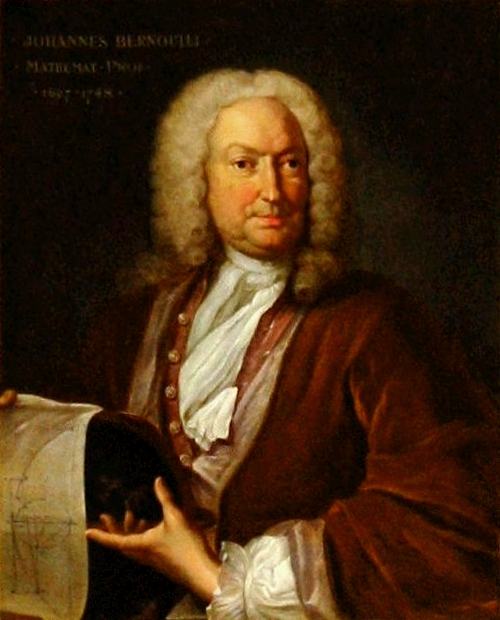
\includegraphics[width=.9\linewidth]{images/Johann_Bernoulli2.jpg}
\caption{Johannes Bernoulli}
\end{figure}
\end{column}
\begin{column}{0.5\columnwidth}
\begin{center}
	\begin{tikzpicture}[baseline,scale=1.2]
	\draw [-latex] (-0.5, 0) -- (4, 0) node [right] {$x$};
	\draw [-latex] (0, 0.5) -- (0, -2) node [below] {$y$};

	%\node [circle,fill=black,inner sep=0pt,minimum size=3pt,label=below:{$\frac{3}{2}$}] (a) at (2/3,0) {};
	\node [anchor = south east] (a) {$A$};

	%\node at (3, -1) [circ] {};
	\node at (3, -1) [right] (b) {$B$};
	\draw [thick, black] (0, 0) parabola bend (2, -1.5) (3, -1);
	\draw [thin, gray, dashed] (0, 0) -- (3, -1);
	\draw [black, fill=black] circle [radius=0.05];
	\draw [black, fill=black] (3,-1) circle [radius=0.05];
	\draw [black, fill=metropolisorange] (0.86, -1) circle [radius=0.1];
	\node at (2, -1.5) [below] {$y = f(x)$};
	\draw [->] (3.8, -0.5) -- (3.8, -1.8) node [below] {$\gv{g}$};
	\end{tikzpicture}
\end{center}
\(\beta \rho \acute{\alpha} \chi \iota \sigma \tau o \varsigma\)
(\emph{brachistos} or shortest) \(\chi
	\rho \acute{o} \nu o \varsigma\) (\emph{chronos} or time)
\end{column}
\end{columns}
\end{frame}
\begin{frame}[label={sec:org9479549}]{Brachistochrone problem}
\begin{columns}
\begin{column}{0.35\columnwidth}
\begin{center}
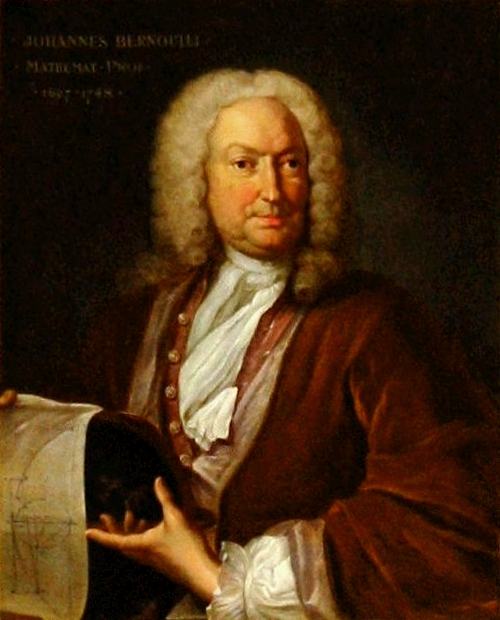
\includegraphics[width=.9\linewidth]{images/Johann_Bernoulli2.jpg}
\end{center}
\end{column}
\begin{column}{0.7\columnwidth}
\begin{quotation} %% :B\_quotation:BMCOL:
{\small ``I, Johann Bernoulli, address the most brilliant mathematicians in the
world..... Following the example set by Pascal, Fermat, etc., I hope to
gain the gratitude of the whole scientific community by placing before the
finest mathematicians of our time a problem which will test their methods and
the strength of their intellect..."}

{\small ``...Given two points A and B in a vertical plane, what is the curve traced out by a
point acted on only by gravity, which starts at A and reaches B in the shortest time."}
\end{quotation}
\end{column}
\end{columns}
\end{frame}

\begin{frame}[label={sec:org205746a}]{Brachistochrone problem : more formally}
\begin{center}
	\begin{tikzpicture}[baseline, scale=0.8]
	\draw [-latex] (-0.5, 0) -- (4, 0) node [right] {$x$};
	\draw [-latex] (0, 0.5) -- (0, -2) node [below] {$y$};

	%\node [circle,fill=black,inner sep=0pt,minimum size=3pt,label=below:{$\frac{3}{2}$}] (a) at (2/3,0) {};
	\node [anchor = south east] (a) {$A$};

	%\node at (3, -1) [circ] {};
	\node at (3, -1) [right] (b) {$B$};
	\draw [thick, black] (0, 0) parabola bend (2, -1.5) (3, -1);
	\draw [thin, gray, dashed] (0, 0) -- (3, -1);
	\draw [black, fill=black] circle [radius=0.05];
	\draw [black, fill=black] (3,-1) circle [radius=0.05];
	\draw [black, fill=metropolisorange] (0.86, -1) circle [radius=0.1];
	\node at (2, -1.5) [below] {$y = f(x)$};
	\draw [->] (3.8, -0.5) -- (3.8, -1.8) node [below] {$\gv{g}$};
	\end{tikzpicture}
\end{center}
\begin{definition}[Brachistochrone problem]
For \(x : [x_A, x_B]\), let
\(\mathbf{x} \mapsto \begin{pmatrix} x \\ y(x) \end{pmatrix},
	 y : [0, x] \to \mathbb{R}\) with BoCos.

Find \(y^*  = \mathop{\mathrm{arg\,min}_y} L[y] \mathrel{\mathop:}= t_B(y, y',y'')\) where
\(t : \mathbb{R}^3 \to \mathbb{R}^+\) is trajectory time.
\begin{block}{In the context of optimization \(\left( \mathcal{C}^2, \mathbb{R}, f, \leq \right)\)}
By solving \(\ddot{x} = \frac{g_x + y' \left[ g_y - y'' \dot{x}^2 \right]}{1 + y'^2}\)
with \(x(A) = x_A, \dot{x}(A) = 0\) to obtain \(x = f(t, y, y', y''')\).
Then \(t \mathrel{\mathop:}= f^{-1}(x, y, y', y''')\)
\end{block}
\end{definition}
\end{frame}
\begin{frame}[label={sec:orgec98416}]{Requirements}
\begin{alertblock}{Simulation}
\begin{itemize}
\item \alert{Numerical solution} of non-linear Ordinary Differential Equation (ODE)
\end{itemize}
\end{alertblock}
\begin{alertblock}{Optimization problem}
\begin{itemize}
\item \alert{Representation} of \(\mathcal{C}^2\)
\item Definition of \alert{fitness function}
\item Black-box \alert{optimizer} (we pick CMAes in this case)
\item \alert{Constraints} on domain and range
\begin{itemize}
\item not all \(\mathcal{C}^2\) are feasible (boundary conditions!)
\end{itemize}
\end{itemize}
\end{alertblock}
\end{frame}
\begin{frame}[label={sec:org3a0642a},fragile]{ODE solver}
 \begin{definition}[Ordinary Differential Equation]
\[ \frac{dy}{dt} = f(t, y, y', \dots, y^{k})\]
accompanied by \(k\) initial conditions \(\Rightarrow\) solved by \(y(t)\).
\begin{itemize}
\item Few non-linear problems can be solved analytically \(\Rightarrow\) \alert{numerical methods}
\item \emph{Timesteppers}---Euler, Runge-Kutta etc.
\end{itemize}
\end{definition}
\begin{example}[Scipy's ODE solver]
\begin{itemize}
\item \texttt{scipy.integrate.odeint} \alert{DEMO}
\item many options \texttt{RK23, RK45, BDF,...}
\item can specify error tolerances \texttt{rtol}, \texttt{atol}
\end{itemize}
\end{example}
\end{frame}
\begin{frame}[label={sec:orgc9d2e0d}]{Representation}
\begin{block}{Function space \(\mathcal{C}^2 \to \mathbb{R}\)?}
\begin{itemize}
\item Our optimizer works ONLY with real numbers
\end{itemize}
\end{block}
\begin{block}{Linear combination of basis functions}
\begin{itemize}
\item \(\forall x \in D\), \(f(x) = \sum_{i=1}^{N} c_i \phi_i(x)\)
\item look for \emph{good} values of \(c_i\)
\end{itemize}
\end{block}
\begin{columns}
\begin{column}{0.32\columnwidth}
\begin{center}
	\begin{tikzpicture}[scale=0.48]
		\begin{axis}[
					title={Polynomial bases},
					xmin=0,
					xmax=1,
					ymin=-1.05,
					ymax=1.05,
					samples=50,
					xlabel={$s$},
					ylabel={$\phi(s)$},
					ylabel shift = -10 pt]
			 \addplot[royalblue,  ultra thick, domain=0:1] {x};
			 \addplot[scarlet, ultra thick, domain=0:1] {x^2};
			 \addplot[black,  ultra thick, domain=0:1] {x^3};
			 \addplot[metropolisorange,  ultra thick, domain=0:1] {x^4};
			 \addplot[shamrockgreen,  ultra thick, domain=0:1] {x^5};
			 \addplot[deeppink,  ultra thick, domain=0:1] {x^6};
			 \addplot[burple,  ultra thick, domain=0:1] {1};
			 \draw[ultra thin] (axis cs:\pgfkeysvalueof{/pgfplots/xmin},0) -- (axis cs:\pgfkeysvalueof{/pgfplots/xmax},0);
		\end{axis}
	\end{tikzpicture}
\end{center}
\end{column}
\begin{column}{0.32\columnwidth}
\begin{center}
	\begin{tikzpicture}[scale=0.48]
		\begin{axis}[
					title={Fourier bases},
					xmin=0,
					xmax=1,
					ymin=-1.05,
					ymax=1.05,
					samples=50,
					xlabel={$s$}]
			\addplot[royalblue, ultra thick, domain=0:1] {sin(deg(pi * x))};
			\addplot[scarlet, ultra thick, domain=0:1] {cos(deg(pi * x))};
			\addplot[black,  ultra thick, domain=0:1] {sin(deg(2.0 * pi * x))};
			\addplot[metropolisorange,  ultra thick, domain=0:1] {cos(deg(2.0 * pi * x)))};
			\addplot[shamrockgreen,  ultra thick, domain=0:1] {sin(deg(3.0 * pi * x))};
			\addplot[deeppink,  ultra thick, domain=0:1] {cos(deg(3.0 * pi * x)))};
			\addplot[burple,  ultra thick, domain=0:1] {1};

			\draw[ultra thin] (axis cs:\pgfkeysvalueof{/pgfplots/xmin},0) -- (axis cs:\pgfkeysvalueof{/pgfplots/xmax},0);
		\end{axis}
	\end{tikzpicture}
\end{center}
\end{column}
\begin{column}{0.32\columnwidth}
\begin{center}
	\begin{tikzpicture}[scale=0.48]
		\begin{axis}[
					title={B-splines},
					xmin=0,
					xmax=1,
					ymin=-1.05,
					ymax=1.05,
					samples=50,
					xlabel={$s$}]
				% Taken from https://pages.mtu.edu/~shene/COURSES/cs3621/NOTES/spline/B-spline/bspline-ex-1.html
				% N02
				\addplot[royalblue, ultra thick, domain=0:0.3] {(1 - (10/3)*x)^2 };

				% N12
				\addplot[scarlet, ultra thick, domain=0:0.3] {(20/3)*(x - (8/3)*x^2)  };
				\addplot[scarlet, ultra thick, domain=0.3:0.5] {2.5*(1.0 - 2*x)^2};

				% N22
				\addplot[black, ultra thick, domain=0:0.3] {(20/3)*x^2  };
				\addplot[black, ultra thick, domain=0.3:0.5] {-3.75 + 25*x - 35*x^2};

				% N32
				\addplot[metropolisorange,  ultra thick, domain=0.3:0.5] {(5*x - 1.5)^2};
				\addplot[metropolisorange,  ultra thick, domain=0.5:0.6] {(6 - 10 * x)^2};

				% N42
				\addplot[shamrockgreen,  ultra thick, domain=0.5:0.6] {20 * (-2 + 7*x - 6*x^2) };
				\addplot[shamrockgreen,  ultra thick, domain=0.6:1] {5*(1 - x)^2};

				% N52
				\addplot[deeppink,  ultra thick, domain=0.5:0.6] {20*x^2 - 20*x + 5 };
				\addplot[deeppink,  ultra thick, domain=0.6:1] {-11.25*x^2 + 17.5*x - 6.25};

				% N52
				\addplot[burple,  ultra thick, domain=0.6:1] {6.25*x^2 - 7.5*x + 2.25};

				\draw[ultra thin] (axis cs:\pgfkeysvalueof{/pgfplots/xmin},0) -- (axis cs:\pgfkeysvalueof{/pgfplots/xmax},0);
		\end{axis}
	\end{tikzpicture}
\end{center}
\end{column}
\end{columns}
\end{frame}
\begin{frame}[label={sec:orgf43b0fc}]{Representation}
\begin{itemize}
\item See\href{http://jsxgraph.uni-bayreuth.de/wiki/index.php/B-splines}{ this link} (B-splines) and \href{https://bl.ocks.org/jinroh/7524988}{this} link + \href{https://www.youtube.com/watch?v=spUNpyF58BY}{this video} for a visual understanding of the different bases functions.
\end{itemize}
\end{frame}
\begin{frame}[label={sec:org36ee4bf}]{Fitness function}
\begin{block}{What's the fitness?}
\begin{itemize}
\item <2-> Measure time at \(x(t) = x_B\)
\end{itemize}
\end{block}
\begin{columns}
\begin{column}{0.3\columnwidth}
\begin{center}
	\begin{tikzpicture}[scale=0.48]
	\begin{axis}[
		grid=major, % Display a grid
		grid style={dashed,gray!30}, % Set the style
		xlabel=$x$, % Set the labels
		% ylabel=$y$,
		ymin=-1.05,
		ymax=0.05
		]
		\node at (axis cs:0,0) [left] (a) {$A$};
		\node at (axis cs:1, -1) [right] (b) {$B$};
		% \draw [black, fill=black] (axis cs:0, 0) circle [radius=0.01];
		% \draw [black, fill=black] (axis cs:1,-1) circle [radius=0.01];
		\addplot[line width=2pt, metropolisorange, mark=none]
		% add a plot from table; you select the columns by using the actual name in
		% the .csv file (on top)
		table[col sep=comma] {data_from_optex/first_spline_profile.csv};
		\addplot[only marks, mark=*]
		table[col sep=comma] {data_from_optex/first_spline_time.csv};
	\end{axis}
	\end{tikzpicture}
\end{center}
\begin{itemize}
\item <2->\(f = \SI{0.638}{\s}\)
\end{itemize}
\end{column}
\begin{column}{0.3\columnwidth}
\begin{center}
	\begin{tikzpicture}[scale=0.48]
	\begin{axis}[
		grid=major, % Display a grid
		grid style={dashed,gray!30}, % Set the style
		xlabel=$x$, % Set the labels
		ymin=-1.05,
		ymax=0.05
		]
		\node at (axis cs:0,0) [left] (a) {$A$};
		\node at (axis cs:1, -1) [right] (b) {$B$};
		% \draw [black, fill=black] (axis cs:0, 0) circle [radius=0.01];
		% \draw [black, fill=black] (axis cs:1,-1) circle [radius=0.01];
		\addplot[line width=2pt, royalblue, mark=none]
		% add a plot from table; you select the columns by using the actual name in
		% the .csv file (on top)
		table[col sep=comma] {data_from_optex/second_spline_profile.csv};
		\addplot[only marks, mark=*]
		table[col sep=comma] {data_from_optex/second_spline_time.csv};
	\end{axis}
	\end{tikzpicture}
\end{center}

\begin{itemize}
\item <2->\(f = \SI{0.713}{\s}\)
\end{itemize}
\end{column}
\begin{column}{0.3\columnwidth}
\begin{center}
	\begin{tikzpicture}[scale=0.48]
	\begin{axis}[
		grid=major, % Display a grid
		grid style={dashed,gray!30}, % Set the style
		xlabel=$x$, % Set the labels
		ymin=-1.05,
		ymax=0.05
		]
		\node at (axis cs:0,0) [left] (a) {$A$};
		\node at (axis cs:1, -1) [right] (b) {$B$};
		% \draw [black, fill=black] (axis cs:0, 0) circle [radius=0.01];
		% \draw [black, fill=black] (axis cs:1,-1) circle [radius=0.01];
		\addplot[line width=2pt, scarlet, mark=none]
		% add a plot from table; you select the columns by using the actual name in
		% the .csv file (on top)
		table[col sep=comma] {data_from_optex/optimal_spline_profile.csv};
		\addplot[only marks, mark=*]
		table[col sep=comma] {data_from_optex/optimal_spline_time.csv};
	\end{axis}
	\end{tikzpicture}
\end{center}
\begin{itemize}
\item <2->\(f = \SI{0.585}{\s}\)
\end{itemize}
\end{column}
\end{columns}
\end{frame}
\begin{frame}[label={sec:orgb1da3ba}]{Constraints and penalties}
\begin{block}{Is unconstrained optimization a good idea?}
\begin{itemize}
\item <2-> \alert{NO}! We penalize \emph{bad} solutions.
\end{itemize}
\end{block}
\begin{columns}
\begin{column}{0.5\columnwidth}
\begin{center}
	\begin{tikzpicture}[scale=0.65]
	\begin{axis}[
		grid=major, % Display a grid
		grid style={dashed,gray!30}, % Set the style
		xlabel=$x$, % Set the labels
		ylabel=$y$,
		ymin=-2.2,
		ymax=0.2
		]
		\node at (axis cs:0,0) [left] (a) {$A$};
		\node at (axis cs:1, -1) [right] (b) {$B$};
		% Different radii because its uneven
		\draw [black, fill=black] (axis cs:0, 0) circle [x radius=0.02, y radius=0.04];
		\draw [black, fill=black] (axis cs:1,-1) circle [x radius=0.02, y radius=0.04];
		\addplot[line width=2pt, scarlet, mark=none]
		% add a plot from table; you select the columns by using the actual name in
		% the .csv file (on top)
		table[col sep=comma] {data_from_optex/positive_slope_spline_profile.csv};
	\end{axis}
	\end{tikzpicture}
\end{center}
\begin{itemize}
\item <2-> Positive slope : simulation \emph{fails}
\end{itemize}
\end{column}
\begin{column}{0.5\columnwidth}
\begin{center}
	\begin{tikzpicture}[scale=0.65]
	\begin{axis}[
		grid=major, % Display a grid
		grid style={dashed,gray!30}, % Set the style
		xlabel=$x$, % Set the labels
		ylabel=$y$,
		ymin=-2.2,
		ymax=0.2
		]
		\node at (axis cs:0,0) [left] (a) {$A$};
		\node at (axis cs:1, -1) [right] (b) {$B$};
		\draw [black, fill=black] (axis cs:0, 0) circle [x radius=0.02, y radius=0.04];
		\draw [black, fill=black] (axis cs:1,-1) circle [x radius=0.02, y radius=0.04];
		\addplot[line width=2pt, royalblue, mark=none]
		% add a plot from table; you select the columns by using the actual name in
		% the .csv file (on top)
		table[col sep=comma] {data_from_optex/third_spline_profile.csv};
		\only<2->{\draw[fill=metropolisorange, fill opacity=0.2] (axis cs:0, 0) rectangle (axis cs:1,-1.3)};
	\end{axis}
	\end{tikzpicture}
\end{center}
\begin{itemize}
\item <2-> Need realistic bounds on coefficients!
\end{itemize}
\end{column}
\end{columns}
\end{frame}
\begin{frame}[label={sec:org2862a29}]{Results}
\href{file:///Users/tp5/code/optex/brachistochrone.mp4}{Brachistochrone optimization}
\end{frame}
\begin{frame}[label={sec:orgd2a3e10}]{Additional discussion}
Think about how these choices affect the optimization campaign?
\begin{block}{Population size / number of generations}
\end{block}
\begin{block}{Number of spline parameters (aka the dimensionality of the problem)?}
\end{block}
\begin{block}{Penalization coefficients?}
\end{block}
\begin{block}{Optimize ``part'' of the problem?}
\end{block}
\begin{block}{Error tolerance of ODE solver?}
\end{block}
\end{frame}
\begin{frame}[label={sec:org4d9f39f}]{Aliters}
\begin{columns}
\begin{column}{0.4\columnwidth}
\begin{block}{Johann's solution}
\begin{itemize}
\item Geometrical
\item Energy conservation
\item Shady (af).
\end{itemize}
\end{block}
\end{column}
\begin{column}{0.6\columnwidth}
\begin{block}{Jakob Bernoulli's solution}
\begin{itemize}
\item Snell's law!
\item Led eventually to calculus of variations
\end{itemize}
\end{block}
\end{column}
\end{columns}
\begin{block}{Isaac Newton's solution}
\begin{itemize}
\item Minimal resistance problem
\end{itemize}
\end{block}
\begin{block}{Calculus of variations / optimal control theory}
\begin{itemize}
\item \(y^*  = \mathop{\mathrm{arg\,min}_y} L[y] \mathrel{\mathop:}=
       \displaystyle\int_{x_A}^{x_B} \dfrac{\sqrt{1 + (y'(x))^2}}{\sqrt{y(x)}}
      dx\)
\end{itemize}
\end{block}
\begin{block}{The optimal solution is a cycloid!}
\end{block}
\end{frame}
\begin{frame}[label={sec:orga1b3307}]{More history\footnote{\href{https://en.wikipedia.org/wiki/Brachistochrone\_curve}{Brachistochrone curve wiki}}}
\footnotesize
\begin{itemize}
\item Johann Bernoulli allowed six months for other solutions (apart from his and
Jakob's)
\item At the request of Leibniz, the time was publicly extended for a year and a
half.
\item At 4 p.m. on 29 January 1697 when he arrived home from the Royal Mint,
Isaac Newton found the challenge in a letter from Johann Bernoulli.
\item Newton stayed up all night to solve it and mailed the solution anonymously
by the next post
\item Upon reading the solution, Bernoulli recognized its author, exclaiming that
he ``recognizes a lion from his claw mark''
\item Johann had taken two weeks to solve the same problem
\item Newton also wrote, ``I do not love to be dunned [pestered] and teased by
foreigners about mathematical things\ldots{}''
\item In the end, five mathematicians responded with solutions: Newton,
Bernoulli(s), Leibniz, Tschirnhaus and l'Hôpital.
\end{itemize}
\end{frame}
\begin{frame}[label={sec:orgb132927}]{Dido's isoperimetric problem\footnote{\href{https://mathematicalgarden.wordpress.com/2008/12/21/the-problem-of-dido/}{Mathematical Garden}}}
\begin{block}{Constraints in the problem definition}
What is the closed curve which has the maximum area for a given perimeter?

\begin{center}
	\begin{tikzpicture}[scale=0.65]
	\begin{axis}[axis equal,
		grid=major, % Display a grid
		grid style={dashed,gray!30}, % Set the style
		xlabel=$x$, % Set the labels
		ylabel=$f(x)$,
		xmin=0,
		xmax=1,
		ymin=0,
		ymax=0.6,
		samples=100]
		\addplot[royalblue,  line width=3pt, domain=0:1] {(0.25-(x-0.5)^2)^0.5};

		\addplot[metropolisorange,  line width=3pt, domain=0:0.5] {2.8*(x-1.5*x^2)};
		\addplot[metropolisorange,  line width=3pt, domain=0.5:1] {1.4*(1-x)^2};

		\addplot[black,  line width=3pt, domain=0.0:0.5] {1.4*x^2};
		\addplot[black,  line width=3pt, domain=0.5:1.0] {2.8*(-0.5-1.5*x^2+2*x)};

	\end{axis}
	\end{tikzpicture}
\end{center}
\end{block}
\end{frame}
\begin{frame}[label={sec:org8a56f7f}]{Results}
\begin{itemize}
\item Constraint satsifaction by pre-processing and not by repair
\item \href{file:///Users/tp5/code/optex/isoperimetric.mp4}{Isoperimetric curve optimization}
\end{itemize}
\end{frame}

\section{Comparing CMA against GA}
\label{sec:org3920800}
\begin{frame}[label={sec:org6553dc1}]{CMAes vs GA--setup}
\begin{block}{Optimization on smooth functions}
\begin{itemize}
\item Two dimensional, \(C^{\infty}\) functions \(f(\gv{x})\) : \(\left(\mathbb{R}^2,  \mathbb{R}, f, \leq \right)\)
\item shifted Schaffer function (optima in the middle well)
\end{itemize}
\end{block}
\begin{center}
	\begin{tikzpicture}[
		declare function={schaffer=0.5 + ((sin(deg(sqrt(x^2+y^2))))^2-0.5)/(1+0.001*(x^2+y^2))^2;}, scale=0.9]
		\begin{axis}[
			colormap name=whitered,
			view={45}{65},
			enlargelimits=false,
			grid=major,
			domain=-8:8,
			y domain=-8:8,
			samples=41,
			xlabel=$x_1$,
			ylabel=$x_2$,
			zlabel={$f_{\text{schaffer}}$},
			colorbar,
		]
		\addplot3 [surf] {schaffer};
		\draw [black!50] (axis cs:-2.5,0,0) -- (axis cs:2.5,0,0);
		\draw [black!50] (axis cs:0,-2.5,0) -- (axis cs:0,2.5,0);
		\end{axis}
	\end{tikzpicture}
\end{center}
\end{frame}
\begin{frame}[label={sec:orgbdacf85}]{CMAes vs GA--setup}
\begin{itemize}
\item shifted Rastrigin function (optima in the middle well)
\begin{center}
	\begin{tikzpicture}[
		declare function={rastrigin=20 + (x^2 - 10*cos(deg(0.85*pi*x))) + (y^2 - 10*cos(deg(0.85*pi*y)));}, scale=1.0]
		\begin{axis}[
			colormap name=whitered,
			view={45}{65},
			enlargelimits=false,
			grid=major,
			domain=-8:8,
			y domain=-8:8,
			samples=41,
			xlabel=$x_1$,
			ylabel=$x_2$,
			zlabel={$f_{\text{rastrigin}}$},
			colorbar,
		]
		\addplot3 [surf] {rastrigin};
		\draw [black!50] (axis cs:-2.5,0,0) -- (axis cs:2.5,0,0);
		\draw [black!50] (axis cs:0,-2.5,0) -- (axis cs:0,2.5,0);
		\end{axis}
	\end{tikzpicture}
\end{center}
\end{itemize}
\end{frame}
\begin{frame}[label={sec:org1dd78b6}]{Comparison between functions\footnote{\href{http://blog.otoro.net/2017/10/29/visual-evolution-strategies/}{Otoro}}}
\begin{columns}
\begin{column}{0.5\columnwidth}
\begin{figure}[htbp]
\centering
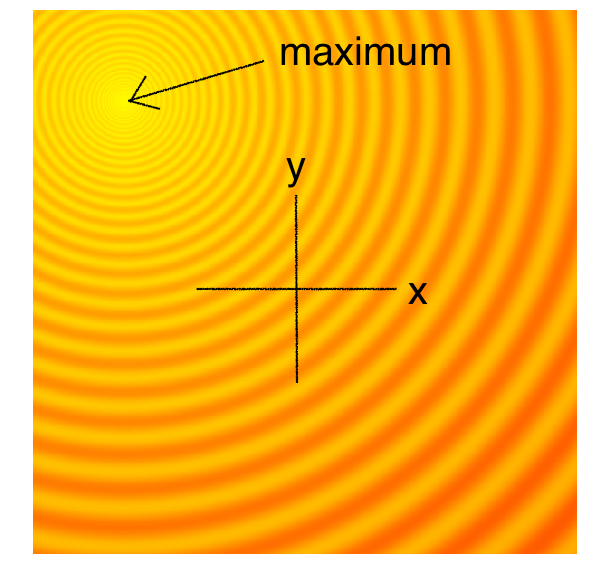
\includegraphics[width=.9\linewidth]{images/schaffer_start.png}
\caption{Schaffer--setup}
\end{figure}
\end{column}
\begin{column}{0.5\columnwidth}
\begin{figure}[htbp]
\centering
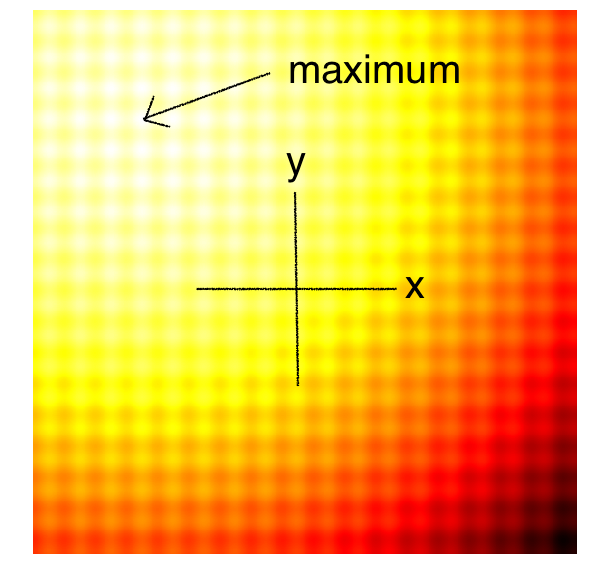
\includegraphics[width=.9\linewidth]{images/rastrigin_start.png}
\caption{Rastrigin--setup}
\end{figure}
\end{column}
\end{columns}

Lighter region indicates smaller values
\end{frame}
\begin{frame}[label={sec:org9a65fcf}]{Simple ES}
\begin{block}{Scheme}
\begin{itemize}
\item \alert{Sampling} : \(\gv{z}_i \sim \mathcal{N}\left( \gv{m}, \bv{C} \right)\)
\item \alert{Mean-update} : \(\gv{m} \leftarrow \gv{z}_{1:\lambda}\)
\item \alert{Covariance-update} : \(\bv{C} = \begin{bmatrix}\sigma^2_x & \sigma_x \sigma_y \\  \sigma_x
      \sigma_y & \sigma^2_y \end{bmatrix}\) \(\sigma_x, \sigma_y\) are fixed.
\item No other updates (on path etc.)
\end{itemize}
\end{block}
\begin{block}{Legend}
\begin{itemize}
\item {\color{shamrockgreen}Green} : Tracks the mean \(\gv{m}\).
\item {\color{royalblue}Blue} : Tracks the sampled solutions
at generetation \(g\).
\item {\color{scarlet}Red} : Tracks the best individual so
far.
\end{itemize}
\end{block}
\begin{block}{Results}
Simple Evolution strategy from \href{http://blog.otoro.net/2017/10/29/visual-evolution-strategies/}{Otoro} shown for 20 generations
\end{block}
\end{frame}
\begin{frame}[label={sec:orgd6f13ea}]{Simple ES-Observations}
\begin{block}{Convergence}
\begin{itemize}
\item What do you expect for general problems?
\item
\end{itemize}
\end{block}
\begin{block}{Rate of convergence}
\begin{itemize}
\item Is this fast/slow convergence?
\item
\end{itemize}
\end{block}
\begin{block}{Number of function evaluations?}
\begin{itemize}
\item High? Low? Not bad?
\item
\end{itemize}
\end{block}
\end{frame}

\begin{frame}[label={sec:org9d40e9b}]{Simple ES-Observations}
\begin{block}{Convergence}
\begin{itemize}
\item What do you expect for general problems?
\item \alert{Will get stuck--lack of diversity, keeps only best population} (See
rastrigin, which temporarily gets stuck)
\item \alert{Heavy} parameter dependence too
\end{itemize}
\end{block}
\begin{block}{Rate of convergence}
\begin{itemize}
\item Is this fast/slow convergence?
\item \alert{Slow--no history information}
\end{itemize}
\end{block}
\begin{block}{Number of function evaluations?}
\begin{itemize}
\item High? Low? Not bad?
\item \alert{Decent--but no promises for real life black-box optimization problems}
\end{itemize}
\end{block}
\end{frame}

\begin{frame}[label={sec:orgc09b9bf}]{Simple GA}
\begin{block}{Scheme}
\begin{itemize}
\item \alert{Environmental selection} : Keep only best \(10 \%\)
\item \alert{Sampling} : Crossover from parents selected above with \(p_c = 1\)
\item \alert{Crossover} : Select two parents, obtain \(x\) or \(y\) from either parent
with \(0.5\) probability (two coin tosses)
\item \alert{Mutation} : Introduce Gaussian noise with fixed \(\sigma\)
\item No other updates (on path etc.)
\end{itemize}
\end{block}
\begin{block}{Legend}
\begin{itemize}
\item {\color{shamrockgreen}Green} : Tracks the elites from
prior generation \(g\).
\item {\color{royalblue}Blue} : Offsprings from candidate solutions.
\item {\color{scarlet}Red} : Tracks the best individual so
far.
\end{itemize}
\end{block}
\end{frame}

\begin{frame}[label={sec:orgc15c83f}]{Simple GA-Observations}
\begin{block}{Convergence}
\begin{itemize}
\item What do you expect for general problems?
\item
\end{itemize}
\end{block}
\begin{block}{Rate of convergence}
\begin{itemize}
\item Is this fast/slow convergence?
\item
\end{itemize}
\end{block}
\begin{block}{Number of function evaluations?}
\begin{itemize}
\item High? Low? Not bad?
\item
\end{itemize}
\end{block}
\end{frame}

\begin{frame}[label={sec:org77008ae}]{Simple GA-Observations}
\begin{block}{Convergence}
\begin{itemize}
\item What do you expect for general problems?
\item \alert{Will get stuck--lack of diversity, keeps only elitist population}
\item \alert{Heavy} parameter dependence
\item \alert{Tracks} modality well (for both Schaffer and Rastrigin)
\end{itemize}
\end{block}
\begin{block}{Rate of convergence}
\begin{itemize}
\item Is this fast/slow convergence?
\item \alert{Slower} than simple ES
\end{itemize}
\end{block}
\begin{block}{Number of function evaluations?}
\begin{itemize}
\item High? Low? Not bad?
\item \alert{High}
\end{itemize}
\end{block}
\end{frame}

\begin{frame}[label={sec:org2c63399}]{CMAes-Observations}
\begin{block}{Can you spot the updates?}
\begin{itemize}
\item \(\gv{m}\) update (fairly obvious)
\item Step size update
\begin{itemize}
\item Path update
\end{itemize}
\item Covariance matrix upfate
\begin{itemize}
\item Rank \(\mu\) updates
\item Rank \(1\) update (Path update)
\end{itemize}
\end{itemize}
\end{block}
\note{:B\_note:
\begin{itemize}
\item Step size : Initially small, As soon as it sees all are moving in one
direction, it quickly adapts in both cases.
\item Step size reduce. Rastrigin more difficult as
optima close to zero, so step size reduce takes time.
\item Cov update : Direction is clearly important. First recognizes the ascent
direction as a prinicpal component. Then of course the next one is
complementary to it\ldots{}
\item Most due to rank \(\mu\) update (as scaling applied there)
\item But rank one update also seen\ldots{}
\end{itemize}}
\end{frame}

\begin{frame}[label={sec:org9b3499d}]{CMAes-Observations}
\begin{block}{Convergence}
\begin{itemize}
\item What do you expect for general problems?
\item \alert{Good} for problems of ``moderate'' dimensions
\end{itemize}
\end{block}
\begin{block}{Rate of convergence}
\begin{itemize}
\item Is this fast/slow convergence?
\item \alert{Fast} (Approximately brackets minima in \(\order{n}\) functional evaluations)
\end{itemize}
\end{block}
\begin{block}{Number of function evaluations?}
\begin{itemize}
\item High? Low? Not bad?
\item Low (same as above)
\end{itemize}
\end{block}
\end{frame}
\begin{frame}[label={sec:orgb3449af}]{CMAes-Some interesting videos}
\begin{itemize}
\item Mario \url{https://www.youtube.com/watch?v=0iipyd7Gi70}
\item Rastrigin : \url{https://www.youtube.com/watch?v=aP31Q7o2UGU}
\item Biped: \url{https://www.youtube.com/watch?v=lOaWvOA9cb4}
\item Robot Invivo: \url{https://www.youtube.com/watch?v=trR2Gc1tLzg}
\item Robot invitro: \url{https://www.youtube.com/watch?v=fjTd06L-9bQ}
\item Knifefish : \url{https://www.youtube.com/watch?v=3XjgZbs0t2g}
\item \url{https://blog.openai.com/evolution-strategies/}
\end{itemize}
\note{:B\_note:
\begin{itemize}
\item Mario video : interesing solutions
\begin{itemize}
\item Why optimal? See what it is doing. It waits for mushroom bullet
\item 0:35 complex paths
\item Stupidity: at 0.02. IT does not wait. Maybe the user programmed for time
to completion too.
\item Stupidit at 0.14 too
\item Waits for bullet at 0.18
\item Waits for bllet at 0.29
\item 0.35 is just awesome
\item Waits for shroom at 0.40
\item Waits for bullet at 0.45, 0.49
\end{itemize}
\end{itemize}}
\end{frame}
\end{document}
